\documentclass[12pt]{book}
\usepackage[a4paper,top=2cm, bottom=2cm, right=1.9cm, left=1.9cm]{geometry}

\usepackage[utf8]{inputenc}
\usepackage{amsmath,amssymb}
\usepackage[dvipsnames]{xcolor}
\usepackage{listings}
\usepackage[hyphens]{url}
\usepackage{graphicx}
\usepackage{tikz}
\usepackage[most]{tcolorbox}
\usepackage{setspace}
\usepackage[skip=10pt plus1pt, indent=0pt]{parskip}
\usepackage{booktabs}
\usepackage{mathtools}
\usepackage{subcaption}
\usepackage{titlesec}
\usepackage{tabularx}
\usepackage{fancyhdr}
\usepackage{float}
\usepackage{enumitem}
\usepackage{array}
\usepackage{xltabular}
\usepackage[nottoc]{tocbibind}
\usepackage[colorlinks=true,linkcolor=black,anchorcolor=black,citecolor=black,filecolor=black,menucolor=black,runcolor=black,urlcolor=black,backref=page]{hyperref}

% Show a placeholder box if an image file is missing.
\newcommand{\safeincludegraphics}[2][]{%
    \IfFileExists{#2}{%
        \includegraphics[#1]{#2}%
    }{%
        \fbox{\parbox[c][4cm][c]{0.8\linewidth}{\centering Missing image\\\texttt{\detokenize{#2}}}}%
    }%
}

% colors
\definecolor{drawgray}{HTML}{666666}
\definecolor{drawgray_l}{HTML}{F5F5F5}
\definecolor{drawblue}{HTML}{6C8EBF}
\definecolor{drawblue_l}{HTML}{DAE8FC}
\definecolor{drawgreen}{HTML}{82B366}
\definecolor{drawgreen_l}{HTML}{D5E8D4}
\definecolor{draworange}{HTML}{D79B00}
\definecolor{draworange_l}{HTML}{FFE6CC}
\definecolor{drawyellow}{HTML}{D6B656}
\definecolor{drawyellow_l}{HTML}{FFF2CC}
\definecolor{drawred}{HTML}{B85450}
\definecolor{drawred_l}{HTML}{EA6B66}
\definecolor{drawviolet}{HTML}{9673A6}
\definecolor{drawviolet_l}{HTML}{E1D5E7}
\definecolor{drawblackish}{HTML}{422222}

\definecolor{deepblue}{rgb}{0,0,0.5}
\definecolor{deepgreen}{rgb}{0,0.5,0}

\lstset{
    language=SQL,
    morekeywords={AFTER, INSTEAD, OF, REFERENCING, FOR, EACH, ROW, DECLARE, IF, TYPE, NEW, RETURNS, SELF, BEGIN, END, CONSTRUCTOR, UNDER, STATIC, INSTANCE, RETURN, OVERRIDING, FINAL, NOT, INSTANTIABLE, UNNEST, MULTISET, ARRAY, COLLECT, METHOD, REF, MEMBER, FUNCTION, PROCEDURE, PRAGMA, RESTRICT_REFERENCES, WNDS, RNDS, TABLE, WITH, ASSIGNMENT, OPTIONS, SCOPE, NESTED, STORE, DEREF, VARRAY, OBJECT, DBMS_OUTPUT, PUT_LINE, INSERTING, UPDATING, THEN, LOOP, EXTEND, TRUNC, DBMS_RANDOM, TO_CHAR, TO_DATE, REPLACE, BEFORE, COMPOUND, OLD, RAISE_APPLICATION_ERROR, SYSDATE, STATEMENT, IS, ROUND, NVL, ELSIF, DUAL, RAWTOHEX, GUID, SYS},
    framesep=1pt,
    xleftmargin=0pt,
    framexleftmargin=0pt,
    frame=tb,
    framerule=1pt,
    basicstyle=\ttfamily\footnotesize,
    keywordstyle=\color{deepblue},
    commentstyle=\color{deepgreen},
    stringstyle=\color{red},
    breaklines=true,
    tabsize=4,
    showstringspaces=false,
    mathescape
}

% 1.15 spacing
\setstretch{1.15}

% Fancy header
\pagestyle{fancy}
\renewcommand{\chaptermark}[1]{\markboth{#1}{}}
\renewcommand{\sectionmark}[1]{\markright{#1}}
\fancyhead{}
\fancyhead[LE]{{\color{black!40}\thepage}}
\fancyhead[RE]{\bfseries\normalfont {\color{black!40}\nouppercase{\rightmark}}}
\fancyhead[LO]{\bfseries\normalfont {\color{black!40}\nouppercase{Chapter \thechapter: \leftmark}}}
\fancyhead[RO]{{\color{black!40}\thepage}}
\setlength{\headheight}{15pt}

% Chapter title
\definecolor{gray75}{gray}{0.75}
\newcommand{\hsp}{\hspace{20pt}}
\titleformat{\chapter}[hang]{\Huge\bfseries}{\selectfont \thechapter\hsp\textcolor{green}{|}\hsp}{0pt}{\Huge\bfseries}

\hypersetup{
    colorlinks=true,
    linkcolor=drawblackish,
    breaklinks=true,
    citecolor=drawblackish,
    urlcolor=drawblue
}

\begin{document}

\begin{titlepage}
  \newgeometry{left=2cm,bottom=0.1cm, right=2cm, top=2cm}
    \begin{center}
        \safeincludegraphics[scale=0.5]{images/uniba-logo.png}\\
        \vspace{0.5cm}
    {\large University of Bari ``Aldo Moro"}\\
    \vspace{0.2cm}
        \vspace{0.5cm}
        {\large Master's Degree in Computer Science}\\
        \hrulefill \\
        \vspace{0.5cm}
        {\large Project Assignment}\\
        \vspace{0.5cm}
        {\large Database Systems}\\
        \vspace{0.5cm}
        {\LARGE \textbf{Database Design and Implementation}}\\
        \vspace{0.4cm}
        {\Large \textbf{StageUp Inc.}}\\
        {\normalsize Audiovisual Equipment Rental \& Installation System}\\

        \vfill
        \begin{tabularx}{\textwidth}{@{}Xr@{}}
          {\large Student:} & {\large \textit{Angelantonio Fedele Murolo}} \\
          {\large Student ID:} & {\large \textit{840167}} \\
        \end{tabularx}
        \textcolor{white}{.}\\
        \vspace{0.5cm}
        \hrulefill \\
        {\large Academic Year 2025/2026}
    \end{center}
\end{titlepage}

\restoregeometry

\tableofcontents
\newpage

\pagestyle{fancy}

\chapter{Conceptual Design}

\subsection{Requirements}

\begin{table}[H]
    \renewcommand{\arraystretch}{1.25}
    \begin{tabularx}{\textwidth}{|X|}
    \hline
    \multicolumn{1}{|c|}{\textbf{``StageUp Inc.''}} \\
    \hline
    The company ``StageUp'' has a central office and several operational depots located across the world, each covering a specific region, which consists of one or more municipalities, where they manage the rental and installation of audiovisual equipment for events. The central office does not handle physical setups. Both the central office and depots are characterized by name, address, city/province, and number of employees. Bookings, either recurring or one-time, are coordinated by the central office. Bookings can be placed by customers via phone, postal mail, email, or through the website. Besides one-time bookings, the company also handles seasonal contracts and special promotional rentals. Bookings are delivered and installed at customer event locations, which are characterized by address, house number, postal code, city, and province. Since each customer can have one or more event locations, each address is identified by a unique code within the customer's profile. Additionally, each event location has a setup time estimate and equipment capacity. Depots have one or more setup teams, each with a maximum number of members. Each team is characterized by an identification code, a name, the number of installations made, and some personal data of its team members. Each booking is characterized by type, date, duration, cost, the team that handled it, and the details of the customer who placed it. Customers, classified as individuals or companies, are identified by an alphanumeric code and their personal details. \\
    \hline
    \end{tabularx}
    \caption{Requirements text}
\end{table}

\subsection{Analysis}

\subsubsection{Reorganization of Concepts}

The concepts can be reorganized as follows:

\begin{table}[H]
    \renewcommand{\arraystretch}{1.25}
    \begin{tabularx}{\textwidth}{|X|}
    \hline
    \multicolumn{1}{|c|}{\textbf{Depot}} \\
    \hline
    StageUp operates several operational depots distributed worldwide. Each depot covers a specific region composed of one or more municipalities, is described by name, address, city/province and number of employees, and organizes one or more setup teams that perform installations. \\
    \hline
    \end{tabularx}
    \caption{Depot's Concepts}
\end{table}

\begin{table}[H]
    \renewcommand{\arraystretch}{1.25}
    \begin{tabularx}{\textwidth}{|X|}
    \hline
    \multicolumn{1}{|c|}{\textbf{Setup Team}} \\
    \hline
    Each depot has one or more setup teams. A setup team is characterized by an identification code, a name, the number of installations made, a maximum number of members, and personal information related to its team members. \\
    \hline
    \end{tabularx}
    \caption{Setup Team's Concepts}
\end{table}

\begin{table}[H]
    \renewcommand{\arraystretch}{1.25}
    \begin{tabularx}{\textwidth}{|X|}
    \hline
    \multicolumn{1}{|c|}{\textbf{Booking}} \\
    \hline
    Bookings are coordinated by the central office and can be recurring or one-time. They can be placed by customers through different channels (phone, postal mail, email, website), and include seasonal contracts and special promotional rentals. Each booking is described by type, date, duration, cost, and by the setup team that handled the service. \\
    \hline
    \end{tabularx}
    \caption{Booking's Concepts}
\end{table}

\begin{table}[H]
    \renewcommand{\arraystretch}{1.25}
    \begin{tabularx}{\textwidth}{|X|}
    \hline
    \multicolumn{1}{|c|}{\textbf{Customer}} \\
    \hline
    Customers place bookings and are classified as individuals or companies. They are identified by an alphanumeric code and their personal details, and each customer can manage one or more event locations where installations are performed. \\
    \hline
    \end{tabularx}
    \caption{Customer's Concepts}
\end{table}

\begin{table}[H]
    \renewcommand{\arraystretch}{1.25}
    \begin{tabularx}{\textwidth}{|X|}
    \hline
    \multicolumn{1}{|c|}{\textbf{Event Location}} \\
    \hline
    Event locations are the places where bookings are delivered and installed. Each location is characterized by address, house number, postal code, city and province; within each customer's profile, every location is identified by a unique code. An event location also stores setup time estimate and equipment capacity. \\
    \hline
    \end{tabularx}
    \caption{Event Location's Concepts}
\end{table}

\subsubsection{Glossary of Terms}

\begin{table}[H]
    \renewcommand{\arraystretch}{1.25}
    \begin{tabularx}{\textwidth}{|X|X|X|X|}
    \hline
    \textbf{Term} & \textbf{Description} & \textbf{Connections} & \textbf{Synonyms} \\
    \hline
    Depot & A StageUp Inc. depot. & Setup Team & Region \\
    \hline
    Setup Team & A team that handles rental and installation. & Depot, Booking & Team \\
    \hline
    Booking & A specific booking placed by a customer on the StageUp Inc. platform. & Customer, Event Location, Setup Team & Rental, Contract \\
    \hline
    Customer & User of the StageUp Inc. platform. & Booking, Event Location & \\
    \hline
    Event Location & One of the different locations of a customer. & Customer, Booking & Address \\
    \hline
    \end{tabularx}
    \caption{Glossary of Terms}
\end{table}

\subsubsection{Level of Abstraction}

At the conceptual level, the term \textbf{Region} is absorbed into \textbf{Depot}. This choice is directly motivated by the track sentence: \emph{``each covering a specific region, which consists of one or more municipalities''}. In this context, region does not introduce an autonomous business object with its own independent lifecycle, but identifies the coverage area of exactly one depot. Therefore, in the conceptual schema, \textbf{Depot} and \textbf{Region} are treated as a single abstraction.

The mention of municipalities is consistent with this decision: municipalities describe the internal composition of the covered region, not an additional core entity required by the current conceptual scope. For this reason, the model keeps \textbf{Depot} as the only main term at this level and postpones detailed territorial representation to the complete ER specification, where needed.

The same abstraction criterion is applied to \textbf{Central Office}. Although explicitly mentioned in the track, central office refers to a single organizational instance of StageUp Inc. and does not represent a plural, independent entity to be managed as a central part of the data model. Since the database is built for StageUp operations and the central office has no operational setup role, introducing a dedicated entity for it would add complexity without modeling benefit. Consequently, Central Office is not included as a standalone entity in the skeleton schema and is treated only as organizational context.

\subsubsection{Entity-Relationship Diagram}

\paragraph{SKELETON SCHEMA} \leavevmode \newline
\begin{figure}[H]
    \centering
    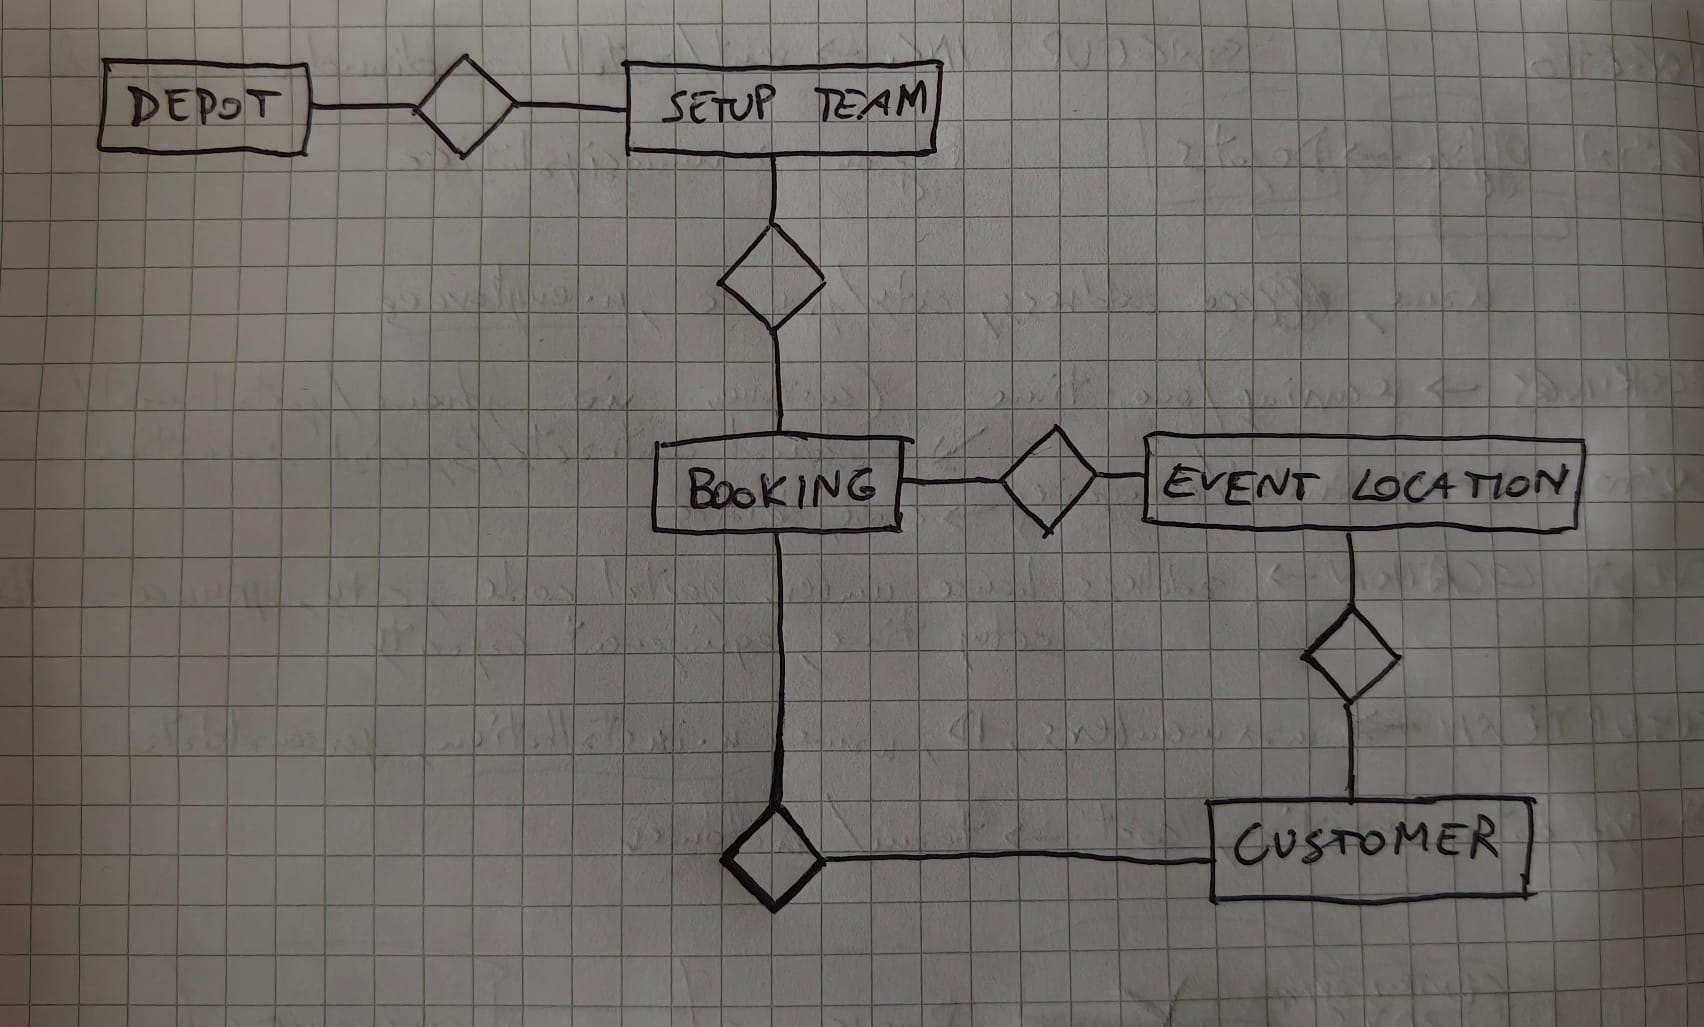
\includegraphics[width=\textwidth]{images/skeleton.jpeg}
    \caption{Skeleton Schema}
\end{figure}

\paragraph{FINAL SCHEMA} \leavevmode \newline
\begin{figure}[H]
    \centering
    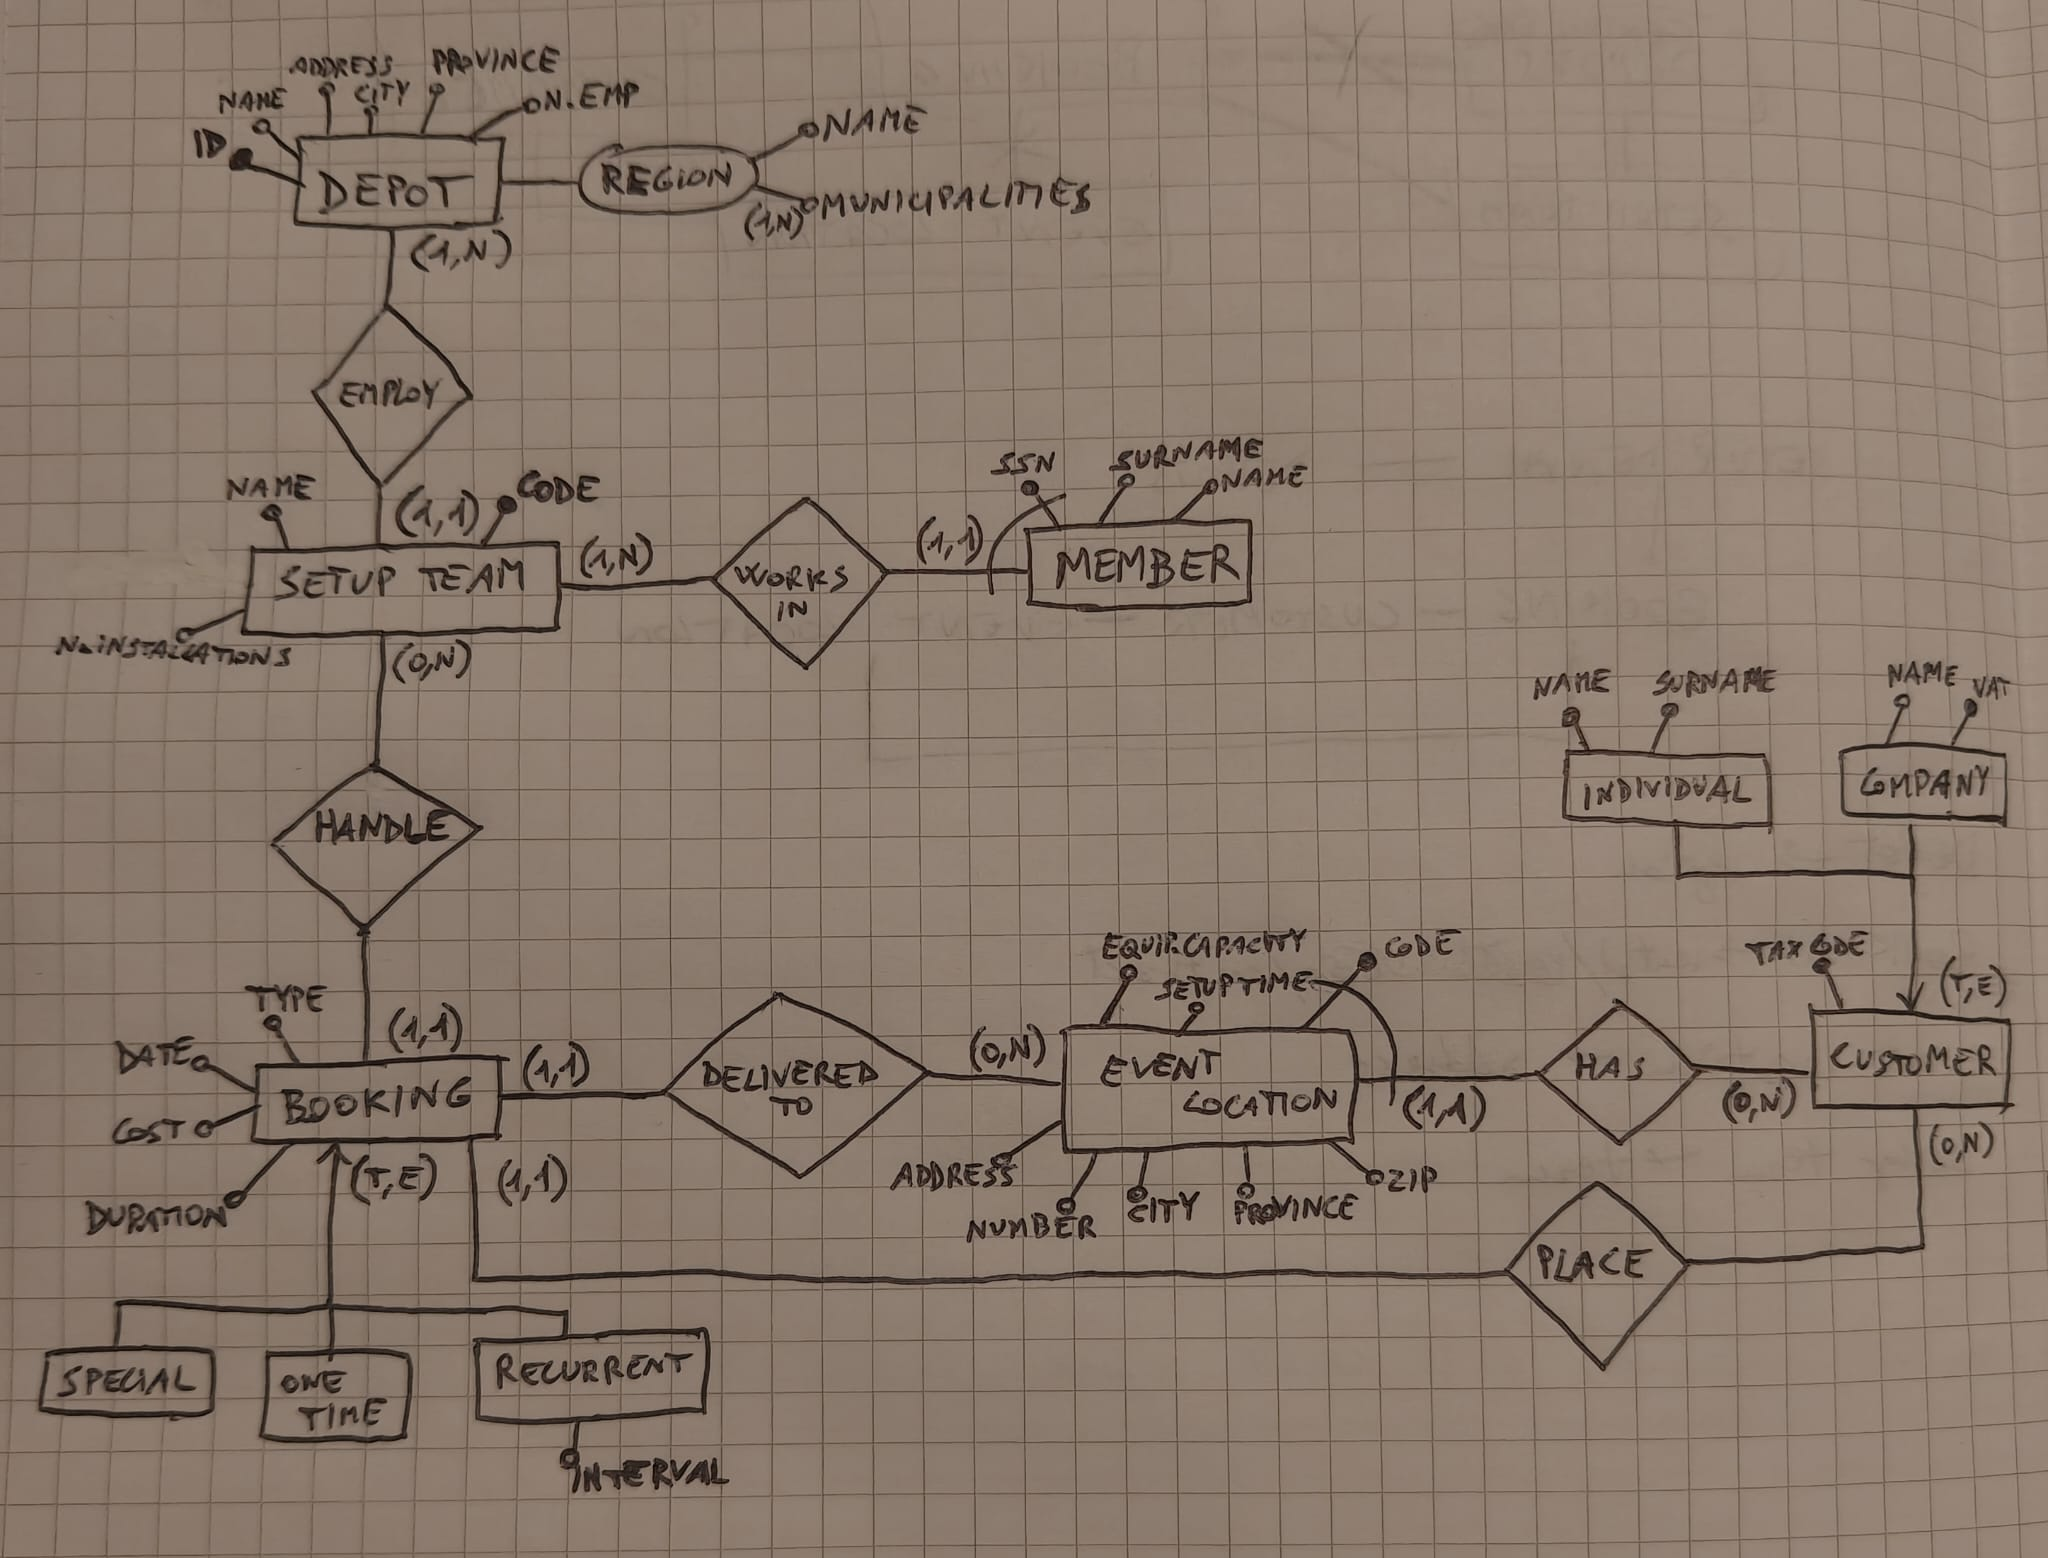
\includegraphics[width=\textwidth]{images/ER FINAL.jpeg}
    \caption{Final Schema}
\end{figure}

\noindent In this final ER schema, \textbf{Region} is not modeled as an autonomous entity; it is represented as a \textbf{composite attribute} of \textbf{Depot}, where \textbf{municipalities} is a \textbf{multivalued attribute}. This modeling choice is consistent with the requirements, since Region does not introduce additional standalone attributes beyond territorial composition. The association between \textbf{Depot} and \textbf{Region} is therefore treated as \textbf{1:1}.

\noindent Conversely, \textbf{Member} is modeled as a proper \textbf{entity}, because the requirements explicitly include personal data (e.g., SSN, name, surname), which should be represented explicitly in the conceptual model. In relation to \textbf{Setup Team}, the cardinality is \textbf{1:N}.

\noindent The attribute \textbf{Max members} has been removed from the \textbf{Setup Team} entity in the ER model, since the track explicitly states that each team may contain at most \textbf{10 members}. For this reason, the limit is treated as a fixed business constraint rather than as a stored attribute.

\subsubsection{Business Rules}
The business rules are the following:
\begin{itemize}
    \item Booking type must be one of \textbf{Phone (P)}, \textbf{Mail (M)}, \textbf{Website (W)}, or \textbf{Email (E)}.
    \item The number of installations of each \textbf{Setup Team} is updated automatically.
    \item A \textbf{Setup Team} can be composed of at most \textbf{10 members}.
    \item A \textbf{Special Booking} is created automatically for the customer and is not placed directly by the customer.
    \item A \textbf{Seasonal Contract} is a \textbf{Recurrent Booking} with a fixed interval of \textbf{4 months}.
\end{itemize}

\chapter{Logical Design}

\section*{Volumes Table}

We consider a one-year observation window for volume estimation.

\begin{table}[H]
    \centering
    \resizebox{\textwidth}{!}{
    \begin{tabular}{|l|c|c|p{9.5cm}|}
    \hline
    \textbf{Concept} & \textbf{Type} & \textbf{Volume} & \textbf{Why} \\
    \hline
    Depot & E & 10 & By specification. \\
    \hline
    Setup Team & E & 100 & By specification. \\
    \hline
    Member & E & 1000 & By specification: each setup team can have at most 10 members, so $100 \cdot 10 = 1000$. \\
    \hline
    Booking & E & 50000 & 1:1 with Place. \\
    \hline
    Special Booking & E & 1000 & Assumption: special rentals are much more occasional than the other booking types. \\
    \hline
    One-Time Booking & E & 40000 & Assumption: one-time bookings are the most frequent booking type. \\
    \hline
    Recurrent Booking & E & 9000 & Assumption: recurrent bookings include seasonal contracts and represent the remaining recurring workload. \\
    \hline
    Event Location & E & 1000 & By specification. \\
    \hline
    Customer & E & 500 & Assumption: each customer has on average at least 2 event locations, so $1000 / 2 = 500$. \\
    \hline
    Individual Customer & E & 400 & Assumption: 4/5 of customers are individuals. \\
    \hline
    Company Customer & E & 100 & Assumption: 1/5 of customers are companies. \\
    \hline
    Employ & R & 100 & 1:1 with Setup Team. \\
    \hline
    Works In & R & 1000 & 1:1 with Member. \\
    \hline
    Handle & R & 50000 & 1:1 with Booking. \\
    \hline
    Delivered To & R & 50000 & 1:1 with Booking. \\
    \hline
    Has & R & 1000 & 1:1 with Event Location. \\
    \hline
    Place & R & 50000 & Assumption: each customer places 100 bookings, so $500 \cdot 100 = 50{,}000$. \\
    \hline
    \end{tabular}
    }
\end{table}

\section*{Operations Table}

The operation set is taken directly from the track.

\begin{table}[H]
    \centering
    \begin{tabular}{|c|c|p{10cm}|c|}
    \hline
    \textbf{Op.} & \textbf{Type} & \textbf{Description} & \textbf{Frequency} \\
    \hline
    1 & I & Enter all data related to a new customer & 10/day \\
    \hline
    2 & I & Record a new booking & 300/day \\
    \hline
    3 & I & Register a new event location & 50/day \\
    \hline
    4 & I & View the team that handled setups at a specific event location & 20/day \\
    \hline
    5 & I & Print event locations sorted by number of bookings (descending) & 5/day \\
    \hline
    \end{tabular}
\end{table}

\section*{Operations Analysis}

\subsection*{Operation 1: Enter all data related to a new customer}

\begin{table}[H]
    \centering
    \begin{tabular}{|l|c|c|c|p{6.3cm}|}
    \hline
    \textbf{Concept} & \textbf{Type} & \textbf{ACC} & \textbf{ACC Type} & \textbf{Why} \\
    \hline
    Customer & E & 1 & W & Create the customer. \\
    \hline
    Event Location & E & 2 & W & Create the two event locations. \\
    \hline
    Customer & E & 1 & R & Read the ID of the newly created customer. \\
    \hline
    Event Location & E & 2 & R & Read the two event locations for the customer. \\
    \hline
    Has & R & 2 & W & Create the two ownership relationships. \\
    \hline
    \end{tabular}
\end{table}

\textbf{Operation cost}: $(2 \cdot (1 + 2 + 2) + (1 + 2)) \cdot 10 = 130$ accesses/day.

\subsection*{Operation 2: Record a new booking}

For creating a new booking, we usually start from the customer ID and the code of the selected event location. Then, based on that location, we identify the setup team that covers the corresponding municipality/area.

Access \textit{without} redundancy:

\begin{table}[H]
    \centering
    \begin{tabular}{|l|c|c|c|p{6.3cm}|}
    \hline
    \textbf{Concept} & \textbf{Type} & \textbf{ACC} & \textbf{ACC Type} & \textbf{Why} \\
    \hline
    Booking & E & 1 & W & Create the booking. \\
    \hline
    Delivered To & R & 1 & W & Create the relationship with the selected event location. \\
    \hline
    Place & R & 1 & W & Create the relationship with the customer. \\
    \hline
    Event Location & E & 1 & R & Read the city/province of the selected event location to identify the serving depot. \\
    \hline
    Depot & E & 10 & R & Find the depot that covers the area of the selected event location. \\
    \hline
    Employ & R & 10 & R & Find the candidate setup teams linked to the selected depot. \\
    \hline
    Handle & R & 1 & W & Create the relationship between booking and selected setup team. \\
    \hline
    \end{tabular}
\end{table}

\textbf{Operation cost} (\textit{without redundancy}): $29 \cdot 300 = 8700$ accesses/day.

Access \textit{with} redundancy:

\begin{table}[H]
    \centering
    \begin{tabular}{|l|c|c|c|p{6.3cm}|}
    \hline
    \textbf{Concept} & \textbf{Type} & \textbf{ACC} & \textbf{ACC Type} & \textbf{Why} \\
    \hline
    Booking & E & 1 & W & Create the booking. \\
    \hline
    Delivered To & R & 1 & W & Create the relationship with the selected event location. \\
    \hline
    Place & R & 1 & W & Create the relationship with the customer. \\
    \hline
    Event Location & E & 1 & R & Read the city/province of the selected event location to identify the serving depot. \\
    \hline
    Depot & E & 10 & R & Find the depot that covers the area of the selected event location. \\
    \hline
    Employ & R & 10 & R & Find the candidate setup teams linked to the selected depot. \\
    \hline
    Setup Team & E & 1 & R & Read the \texttt{n. Installations} of the selected setup team. \\
    \hline
    Setup Team & E & 1 & W & Update the \texttt{n. Installations} for the selected setup team. \\
    \hline
    Handle & R & 1 & W & Create the relationship between booking and selected setup team. \\
    \hline
    \end{tabular}
\end{table}

\textbf{Operation cost} (\textit{with redundancy}): $32 \cdot 300 = 9600$ accesses/day.

\subsection*{Operation 3: Register a new event location}

For registering a new event location, we usually already have the customer ID, since the customer must be authenticated before adding a location.

\begin{table}[H]
    \centering
    \begin{tabular}{|l|c|c|c|p{6.3cm}|}
    \hline
    \textbf{Concept} & \textbf{Type} & \textbf{ACC} & \textbf{ACC Type} & \textbf{Why} \\
    \hline
    Event Location & E & 1 & W & Create the event location. \\
    \hline
    Has & R & 1 & W & Create the relationship with the customer. \\
    \hline
    \end{tabular}
\end{table}

\textbf{Operation cost}: $4 \cdot 50 = 200$ accesses/day.

\subsection*{Operation 4: View the team that handled setups at a specific event location}

\begin{table}[H]
    \centering
    \begin{tabular}{|l|c|c|c|p{6.3cm}|}
    \hline
    \textbf{Concept} & \textbf{Type} & \textbf{ACC} & \textbf{ACC Type} & \textbf{Why} \\
    \hline
    Event Location & E & 1 & R & Read the ID of the selected event location. \\
    \hline
    Delivered To & R & 50 & R & Average of 50 bookings per location: $50000 / 1000 = 50$. \\
    \hline
    Booking & E & 50 & R & 1:1 with Delivered To, one booking for each delivered-to instance. \\
    \hline
    Handle & R & 50 & R & 1:1 with Booking, retrieve the team relation for each booking. \\
    \hline
    \end{tabular}
\end{table}

\textbf{Operation cost}: $151 \cdot 20 = 3020$ accesses/day.

\subsection*{Operation 5: Print event locations sorted by number of bookings}

\begin{table}[H]
    \centering
    \begin{tabular}{|l|c|c|c|p{6.3cm}|}
    \hline
    \textbf{Concept} & \textbf{Type} & \textbf{ACC} & \textbf{ACC Type} & \textbf{Why} \\
    \hline
    Delivered To & R & 50000 & R & Read all relationship instances to count occurrences of each event location ID. \\
    \hline
    Event Location & E & 1000 & R & Access and print the actual event location data. \\
    \hline
    \end{tabular}
\end{table}

\textbf{Operation cost}: $(50000 + 1000) \cdot 5 = 255000$ accesses/day.

\section*{Design Considerations}

In this section, redundancy and generalization situations are analyzed.

\subsection*{Setup Team n. Installations}

The attribute \texttt{n. Installations} in \texttt{Setup Team} is removed from the logical baseline as a stored redundancy. The comparison on Operation 2 shows that maintaining this counter increases write cost (additional read/write on setup team), while none of the required operations explicitly needs that value as direct output.

\subsection*{Relation Place (Customer-Booking)}

The relation \texttt{Place} is redundant, because customer information is still reachable through \texttt{Has} (Customer-Event Location) together with \texttt{Delivered To} (Booking-Event Location).

\textbf{Operation 2 with \texttt{Place}} (original table):

\begin{table}[H]
    \centering
    \begin{tabular}{|l|c|c|c|p{6.3cm}|}
    \hline
    \textbf{Concept} & \textbf{Type} & \textbf{ACC} & \textbf{ACC Type} & \textbf{Why} \\
    \hline
    Booking & E & 1 & W & Create the booking. \\
    \hline
    Delivered To & R & 1 & W & Create the relationship with the selected event location. \\
    \hline
    Place & R & 1 & W & Create the relationship with the customer. \\
    \hline
    Event Location & E & 1 & R & Read the city/province of the selected event location to identify the serving depot. \\
    \hline
    Depot & E & 10 & R & Find the depot that covers the area of the selected event location. \\
    \hline
    Employ & R & 10 & R & Find the candidate setup teams linked to the selected depot. \\
    \hline
    Handle & R & 1 & W & Create the relationship between booking and selected setup team. \\
    \hline
    \end{tabular}
\end{table}

\textbf{Operation 2 with \texttt{Has} replacing \texttt{Place}}:

\begin{table}[H]
    \centering
    \begin{tabular}{|l|c|c|c|p{6.3cm}|}
    \hline
    \textbf{Concept} & \textbf{Type} & \textbf{ACC} & \textbf{ACC Type} & \textbf{Why} \\
    \hline
    Booking & E & 1 & W & Create the booking. \\
    \hline
    Delivered To & R & 1 & W & Create the relationship with the selected event location. \\
    \hline
    \textbf{Has} & \textbf{R} & \textbf{1} & \textbf{R} & \textbf{Check customer ownership of the selected event location (replacement row).} \\
    \hline
    Event Location & E & 1 & R & Read the city/province of the selected event location to identify the serving depot. \\
    \hline
    Depot & E & 10 & R & Find the depot that covers the area of the selected event location. \\
    \hline
    Employ & R & 10 & R & Find the candidate setup teams linked to the selected depot. \\
    \hline
    Handle & R & 1 & W & Create the relationship between booking and selected setup team. \\
    \hline
    \end{tabular}
\end{table}

\[
\text{With Place: } (2 \cdot 4 + 21) \cdot 300 = 29 \cdot 300 = 8700\ \text{accesses/day}
\]
\[
\text{With Has replacement: } (2 \cdot 3 + 22) \cdot 300 = 28 \cdot 300 = 8400\ \text{accesses/day}
\]

\noindent The replacement preserves functionality and slightly reduces weighted accesses, so \texttt{Place} is removed from the logical restructuring.

\subsection*{Partitioning and Merging Choices}

For \texttt{Booking}, the specialization (Special / One-Time / Recurrent) is collapsed into a single entity. The entity keeps standard booking attributes and introduces:

\begin{itemize}
    \item a boolean \texttt{IsSpecial};
    \item an \texttt{Interval} attribute for recurrent behavior.
\end{itemize}

Interpretation rule:

\begin{itemize}
    \item if \texttt{IsSpecial = TRUE}, the booking is a special rental;
    \item if \texttt{Interval} is greater than zero, the booking is recurrent.
\end{itemize}

For \texttt{Customer}, specialization is maintained, because \texttt{Individual} and \texttt{Company} have distinct, non-overlapping attributes.

\subsection*{Event Location Identifier After Place Removal}

After removing \texttt{Place}, \texttt{Event Location} is treated with an autonomous unique code (no longer customer-scoped). This keeps the \texttt{Booking}-\texttt{Event Location} connection independent and supports the replacement of \texttt{Place} with the \texttt{Delivered To} + \texttt{Has} navigation path.

\section*{UML Schema}

The following UML schema summarizes the final logical structure adopted in this chapter.

\begin{figure}[H]
    \centering
    \safeincludegraphics[width=0.92\textwidth]{images/UMLFINAL.png}
    \caption{UML Schema}
\end{figure}








\chapter{Implementation}

This chapter presents the Oracle object-relational implementation derived from the final logical design and UML schema.

\section{Types Definition}


\begin{lstlisting}
CREATE OR REPLACE TYPE MunicipalityListTY AS TABLE OF VARCHAR2(80);
/
\end{lstlisting}

\begin{lstlisting}
CREATE OR REPLACE TYPE DepotTY AS OBJECT (
    ID            VARCHAR2(20),
    Name          VARCHAR2(100),
    Address       VARCHAR2(100),
    City          VARCHAR2(50),
    Province      VARCHAR2(50),
    N_Emp         NUMBER,
    CoveredRegion VARCHAR2(80),
    Municipalities MunicipalityListTY
);
/
\end{lstlisting}

\begin{lstlisting}
CREATE OR REPLACE TYPE MemberTY AS OBJECT (
    SSN     VARCHAR2(16),
    Name    VARCHAR2(50),
    Surname VARCHAR2(50)
);
/

CREATE OR REPLACE TYPE MemberListTY AS TABLE OF MemberTY;
/

CREATE OR REPLACE TYPE SetupTeamTY AS OBJECT (
    Code    VARCHAR2(20),
    Name    VARCHAR2(100),
    Depot   REF DepotTY,
    Members MemberListTY
);
/
\end{lstlisting}

\begin{lstlisting}
CREATE OR REPLACE TYPE CustomerTY AS OBJECT (
    TaxCode       VARCHAR2(20),
    CustomerType  VARCHAR2(20),
    FirstName     VARCHAR2(50),
    LastName      VARCHAR2(50),
    VAT           VARCHAR2(20),
    CompanyName   VARCHAR2(100)
);
/
\end{lstlisting}

\begin{lstlisting}
CREATE OR REPLACE TYPE EventLocationTY AS OBJECT (
    Code     VARCHAR2(20),
    Address  VARCHAR2(100),
    NumberH  NUMBER,
    City     VARCHAR2(50),
    Prov     VARCHAR2(50),
    ZIP      VARCHAR2(10),
    Customer REF CustomerTY
);
/
\end{lstlisting}

\begin{lstlisting}
CREATE OR REPLACE TYPE BookingTY AS OBJECT (
    Code          VARCHAR2(20),
    Type          CHAR(1),
    Cost          NUMBER(10,2),
    BookDate      DATE,
    IntervalM     NUMBER,
    IsSpecial     CHAR(1),
    Team          REF SetupTeamTY,
    EventLocation REF EventLocationTY
);
/
\end{lstlisting}


\section{Tables Definition}


\begin{lstlisting}
CREATE TABLE DEPOT OF DepotTY (
    ID PRIMARY KEY,
    Name NOT NULL,
    Address NOT NULL,
    City NOT NULL,
    Province NOT NULL,
    N_Emp CHECK (N_Emp >= 0)
)
NESTED TABLE Municipalities STORE AS DepotMunicipalitiesNT;
\end{lstlisting}

\begin{lstlisting}
CREATE TABLE SETUPTEAM OF SetupTeamTY (
    Code PRIMARY KEY,
    Name NOT NULL,
    Depot NOT NULL REFERENCES DEPOT
)
NESTED TABLE Members STORE AS SetupTeamMembersNT;
\end{lstlisting}

\begin{lstlisting}
CREATE TABLE CUSTOMER OF CustomerTY (
    TaxCode PRIMARY KEY,
    CustomerType NOT NULL CHECK (CustomerType IN ('individual', 'company')),
    VAT UNIQUE,
    CHECK (
        (CustomerType = 'individual'
            AND FirstName IS NOT NULL
            AND LastName IS NOT NULL
            AND VAT IS NULL
            AND CompanyName IS NULL)
        OR
        (CustomerType = 'company'
            AND VAT IS NOT NULL
            AND CompanyName IS NOT NULL
            AND FirstName IS NULL
            AND LastName IS NULL)
    )
);
\end{lstlisting}

\begin{lstlisting}
CREATE TABLE EVENTLOCATION OF EventLocationTY (
    Code PRIMARY KEY,
    Address NOT NULL,
    NumberH CHECK (NumberH > 0),
    City NOT NULL,
    Prov NOT NULL,
    ZIP NOT NULL,
    Customer NOT NULL REFERENCES CUSTOMER ON DELETE CASCADE
);
\end{lstlisting}

\begin{lstlisting}
CREATE TABLE BOOKING OF BookingTY (
    Code PRIMARY KEY,
    Type NOT NULL CHECK (Type IN ('P','M','E','W')),
    Cost NOT NULL CHECK (Cost >= 0),
    BookDate NOT NULL,
    IntervalM NOT NULL CHECK (IntervalM >= 0),
    IsSpecial NOT NULL CHECK (IsSpecial IN ('Y','N')),
    Team NOT NULL REFERENCES SETUPTEAM,
    EventLocation NOT NULL REFERENCES EVENTLOCATION
);
\end{lstlisting}

\section{Trigger Implementation}


\subsection*{CheckCustomerType}
Enforces total and exclusive specialization for customers.

\begin{lstlisting}
CREATE OR REPLACE TRIGGER trg_check_customer_type
BEFORE INSERT OR UPDATE ON CUSTOMER
FOR EACH ROW
BEGIN
    IF :NEW.CustomerType = 'individual' THEN
        IF :NEW.FirstName IS NULL OR :NEW.LastName IS NULL THEN
            RAISE_APPLICATION_ERROR(-20001, 'Individual customer requires first and last name');
        END IF;
        IF :NEW.VAT IS NOT NULL OR :NEW.CompanyName IS NOT NULL THEN
            RAISE_APPLICATION_ERROR(-20002, 'Individual customer cannot have company data');
        END IF;
    ELSIF :NEW.CustomerType = 'company' THEN
        IF :NEW.VAT IS NULL OR :NEW.CompanyName IS NULL THEN
            RAISE_APPLICATION_ERROR(-20003, 'Company customer requires VAT and company name');
        END IF;
        IF :NEW.FirstName IS NOT NULL OR :NEW.LastName IS NOT NULL THEN
            RAISE_APPLICATION_ERROR(-20004, 'Company customer cannot have personal name data');
        END IF;
    ELSE
        RAISE_APPLICATION_ERROR(-20005, 'Invalid customer type');
    END IF;
END;
/
\end{lstlisting}

\subsection*{CheckDepotMunicipalities}
Guarantees that each depot covers at least one municipality.

\begin{lstlisting}
CREATE OR REPLACE TRIGGER trg_check_depot_municipalities
BEFORE INSERT OR UPDATE ON DEPOT
FOR EACH ROW
BEGIN
    IF :NEW.Municipalities IS NULL OR :NEW.Municipalities.COUNT = 0 THEN
        RAISE_APPLICATION_ERROR(-20006, 'Depot must include at least one municipality');
    END IF;
END;
/
\end{lstlisting}

\subsection*{CheckTeamMembers}
Enforces composition cardinality \texttt{SetupTeam 1 *-- 0..10 Member} and uniqueness of member SSN within each team.

\begin{lstlisting}
CREATE OR REPLACE TRIGGER trg_check_team_members
BEFORE INSERT OR UPDATE ON SETUPTEAM
FOR EACH ROW
DECLARE
    v_dup NUMBER;
BEGIN
    IF :NEW.Members IS NOT NULL AND :NEW.Members.COUNT > 10 THEN
        RAISE_APPLICATION_ERROR(-20007, 'A setup team cannot contain more than 10 members');
    END IF;

    IF :NEW.Members IS NOT NULL THEN
        SELECT COUNT(*)
        INTO v_dup
        FROM (
            SELECT m.SSN
            FROM TABLE(:NEW.Members) m
            GROUP BY m.SSN
            HAVING COUNT(*) > 1
        );

        IF v_dup > 0 THEN
            RAISE_APPLICATION_ERROR(-20008, 'Duplicate member SSN in the same setup team');
        END IF;
    END IF;
END;
/
\end{lstlisting}

\subsection*{CheckBookingOverlap}
Prevents overlapping booking windows for the same setup team.

\begin{lstlisting}
CREATE OR REPLACE TRIGGER trg_check_booking_overlap
BEFORE INSERT OR UPDATE ON BOOKING
FOR EACH ROW
DECLARE
    v_overlap NUMBER;
BEGIN
    SELECT COUNT(*)
    INTO v_overlap
    FROM BOOKING b
    WHERE b.Team = :NEW.Team
      AND b.Code <> NVL(:OLD.Code, '###')
      AND :NEW.BookDate <= b.BookDate + b.IntervalM
      AND b.BookDate <= :NEW.BookDate + :NEW.IntervalM;

    IF v_overlap > 0 THEN
        RAISE_APPLICATION_ERROR(-20009, 'Team already assigned in an overlapping time window');
    END IF;
END;
/
\end{lstlisting}

\subsection*{CheckBookingEventLocationCustomer}
Ensures that each booking references an event location that is effectively linked to an existing customer profile.

\begin{lstlisting}
CREATE OR REPLACE TRIGGER trg_booking_eventlocation_customer_match
BEFORE INSERT OR UPDATE ON BOOKING
FOR EACH ROW
DECLARE
    v_location EventLocationTY;
    v_customer CustomerTY;
BEGIN
    IF :NEW.EventLocation IS NULL THEN
        RAISE_APPLICATION_ERROR(-20010, 'Booking must reference an event location');
    END IF;

    SELECT DEREF(:NEW.EventLocation)
    INTO v_location
    FROM DUAL;

    IF v_location IS NULL OR v_location.Customer IS NULL THEN
        RAISE_APPLICATION_ERROR(-20011, 'Event location must be linked to a customer');
    END IF;

    SELECT DEREF(v_location.Customer)
    INTO v_customer
    FROM DUAL;

    IF v_customer IS NULL THEN
        RAISE_APPLICATION_ERROR(-20012, 'Referenced customer does not exist');
    END IF;
END;
/
\end{lstlisting}

\subsection*{CheckBookingDateNotPast}
Blocks inserts and updates when the booking date is in the past.

\begin{lstlisting}
CREATE OR REPLACE TRIGGER trg_booking_date_not_past
BEFORE INSERT OR UPDATE ON BOOKING
FOR EACH ROW
BEGIN
    IF :NEW.BookDate < TRUNC(SYSDATE) THEN
        RAISE_APPLICATION_ERROR(-20013, 'Booking date cannot be in the past');
    END IF;
END;
/
\end{lstlisting}

\subsection*{LockPastBookingReassignment}
Prevents team or destination location reassignment for historical bookings.

\begin{lstlisting}
CREATE OR REPLACE TRIGGER trg_lock_past_booking_reassignment
BEFORE UPDATE OF Team, EventLocation ON BOOKING
FOR EACH ROW
BEGIN
    IF :OLD.BookDate < TRUNC(SYSDATE)
       AND (:OLD.Team <> :NEW.Team OR :OLD.EventLocation <> :NEW.EventLocation) THEN
        RAISE_APPLICATION_ERROR(-20014, 'Team or location cannot be changed for past bookings');
    END IF;
END;
/
\end{lstlisting}

\section{Database Population}

Data generation is organized into modular procedures, one per logical area, plus a final orchestration procedure.

\subsection*{populateDepot}

\begin{lstlisting}
CREATE OR REPLACE PROCEDURE populateDepot(p_num_depots IN NUMBER) AS
    v_emp_count NUMBER;
BEGIN
    FOR d IN 1 .. p_num_depots LOOP
        v_emp_count := TRUNC(DBMS_RANDOM.VALUE(8, 60));

        INSERT INTO DEPOT VALUES (
            DepotTY(
                'D' || TO_CHAR(d, 'FM000'),
                'Depot ' || DBMS_RANDOM.STRING('U', 6),
                'Street ' || DBMS_RANDOM.STRING('U', 8),
                'City ' || DBMS_RANDOM.STRING('U', 6),
                'PR' || TO_CHAR(MOD(d, 20), 'FM00'),
                v_emp_count,
                'Region ' || DBMS_RANDOM.STRING('U', 5),
                MunicipalityListTY(
                    'Municipality ' || DBMS_RANDOM.STRING('U', 6),
                    'Municipality ' || DBMS_RANDOM.STRING('U', 6),
                    'Municipality ' || DBMS_RANDOM.STRING('U', 6)
                )
            )
        );
    END LOOP;
END;
/
\end{lstlisting}

\subsection*{populateSetupTeam}

\begin{lstlisting}
CREATE OR REPLACE PROCEDURE populateSetupTeam(p_num_teams_per_depot IN NUMBER) AS
    v_team_code    VARCHAR2(20);
    v_members      MemberListTY;
    v_member_count NUMBER;
BEGIN
    FOR d IN (SELECT ID FROM DEPOT ORDER BY ID) LOOP
        FOR t IN 1 .. p_num_teams_per_depot LOOP
            v_team_code := 'T' || SUBSTR(d.ID, 2) || '_' || TO_CHAR(t, 'FM00');
            v_members := MemberListTY();
            v_member_count := TRUNC(DBMS_RANDOM.VALUE(0, 11));

            FOR m IN 1 .. v_member_count LOOP
                v_members.EXTEND;
                v_members(v_members.COUNT) := MemberTY(
                    'SSN' || TO_CHAR(TO_NUMBER(SUBSTR(d.ID, 2)) * 10000 + t * 100 + m, 'FM0000000'),
                    'Name' || DBMS_RANDOM.STRING('U', 7),
                    'Surname' || DBMS_RANDOM.STRING('U', 7)
                );
            END LOOP;

            INSERT INTO SETUPTEAM VALUES (
                SetupTeamTY(
                    v_team_code,
                    'Team ' || DBMS_RANDOM.STRING('U', 6),
                    (SELECT REF(dp) FROM DEPOT dp WHERE dp.ID = d.ID),
                    v_members
                )
            );
        END LOOP;
    END LOOP;
END;
/
\end{lstlisting}

\subsection*{populateCustomer}

\begin{lstlisting}
CREATE OR REPLACE PROCEDURE populateCustomer(p_num_customers IN NUMBER) AS
BEGIN
    FOR c IN 1 .. p_num_customers LOOP
        IF DBMS_RANDOM.VALUE(0, 1) < 0.6 THEN
            INSERT INTO CUSTOMER VALUES (
                CustomerTY(
                    'C' || TO_CHAR(c, 'FM0000'),
                    'individual',
                    'Name' || DBMS_RANDOM.STRING('U', 8),
                    'Surname' || DBMS_RANDOM.STRING('U', 8),
                    NULL,
                    NULL
                )
            );
        ELSE
            INSERT INTO CUSTOMER VALUES (
                CustomerTY(
                    'C' || TO_CHAR(c, 'FM0000'),
                    'company',
                    NULL,
                    NULL,
                    'VAT' || TO_CHAR(c, 'FM000000000'),
                    'Company ' || DBMS_RANDOM.STRING('U', 8)
                )
            );
        END IF;
    END LOOP;
END;
/
\end{lstlisting}

\subsection*{populateEventLocation}

\begin{lstlisting}
CREATE OR REPLACE PROCEDURE populateEventLocation(p_num_locations_per_customer IN NUMBER) AS
    v_location_code VARCHAR2(20);
BEGIN
    FOR c IN (SELECT TaxCode FROM CUSTOMER ORDER BY TaxCode) LOOP
        FOR l IN 1 .. p_num_locations_per_customer LOOP
            v_location_code := 'L' || SUBSTR(c.TaxCode, 2) || '_' || TO_CHAR(l, 'FM00');

            INSERT INTO EVENTLOCATION VALUES (
                EventLocationTY(
                    v_location_code,
                    'Address ' || DBMS_RANDOM.STRING('U', 10),
                    TRUNC(DBMS_RANDOM.VALUE(1, 300)),
                    'City ' || DBMS_RANDOM.STRING('U', 6),
                    'PR' || TO_CHAR(MOD(TO_NUMBER(SUBSTR(c.TaxCode, 2)), 20), 'FM00'),
                    'ZIP' || TO_CHAR(TRUNC(DBMS_RANDOM.VALUE(10000, 99999))),
                    (SELECT REF(cu) FROM CUSTOMER cu WHERE cu.TaxCode = c.TaxCode)
                )
            );
        END LOOP;
    END LOOP;
END;
/
\end{lstlisting}

\subsection*{populateBooking}

\begin{lstlisting}
CREATE OR REPLACE PROCEDURE populateBooking(p_num_bookings IN NUMBER) AS
    TYPE refTeamTab IS TABLE OF REF SetupTeamTY INDEX BY PLS_INTEGER;
    TYPE refLocTab  IS TABLE OF REF EventLocationTY INDEX BY PLS_INTEGER;
    TYPE numTab     IS TABLE OF NUMBER INDEX BY PLS_INTEGER;
    teams      refTeamTab;
    locations  refLocTab;
    v_last_end numTab;
    v_t_idx    PLS_INTEGER;
    v_l_idx    PLS_INTEGER;
    v_type     CHAR(1);
    v_interval NUMBER;
    v_start    NUMBER;
    v_rand     NUMBER;
BEGIN
    SELECT REF(t) BULK COLLECT INTO teams FROM SETUPTEAM t;
    SELECT REF(l) BULK COLLECT INTO locations FROM EVENTLOCATION l;

    FOR i IN 1 .. teams.COUNT LOOP
        v_last_end(i) := 0;
    END LOOP;

    FOR b IN 1 .. p_num_bookings LOOP
        v_t_idx := TRUNC(DBMS_RANDOM.VALUE(1, teams.COUNT + 1));
        v_l_idx := TRUNC(DBMS_RANDOM.VALUE(1, locations.COUNT + 1));

        v_rand := DBMS_RANDOM.VALUE(0, 1);
        IF v_rand < 0.25 THEN
            v_type := 'P';
        ELSIF v_rand < 0.50 THEN
            v_type := 'M';
        ELSIF v_rand < 0.75 THEN
            v_type := 'E';
        ELSE
            v_type := 'W';
        END IF;

        v_interval := TRUNC(DBMS_RANDOM.VALUE(0, 4));
        v_start := v_last_end(v_t_idx) + 1 + TRUNC(DBMS_RANDOM.VALUE(0, 3));
        v_last_end(v_t_idx) := v_start + v_interval;

        INSERT INTO BOOKING VALUES (
            BookingTY(
                'B' || TO_CHAR(b, 'FM000000'),
                v_type,
                ROUND(DBMS_RANDOM.VALUE(80, 1200), 2),
                TRUNC(SYSDATE) + v_start,
                v_interval,
                CASE WHEN DBMS_RANDOM.VALUE(0, 1) < 0.3 THEN 'Y' ELSE 'N' END,
                teams(v_t_idx),
                locations(v_l_idx)
            )
        );
    END LOOP;
END;
/
\end{lstlisting}

\begin{lstlisting}
CREATE OR REPLACE PROCEDURE PopulateDatabase(
    p_num_depots                  IN NUMBER,
    p_num_teams_per_depot         IN NUMBER,
    p_num_customers               IN NUMBER,
    p_num_locations_per_customer  IN NUMBER,
    p_num_bookings                IN NUMBER
)
AS
BEGIN
    populateDepot(p_num_depots);
    populateSetupTeam(p_num_teams_per_depot);
    populateCustomer(p_num_customers);
    populateEventLocation(p_num_locations_per_customer);
    populateBooking(p_num_bookings);
END;
/
\end{lstlisting}

\begin{lstlisting}
BEGIN
    DBMS_OUTPUT.PUT_LINE('Starting StageUp population...');
    PopulateDatabase(
        p_num_depots                 => 10,
        p_num_teams_per_depot        => 10,
        p_num_customers              => 500,
        p_num_locations_per_customer => 2,
        p_num_bookings               => 50000
    );
    DBMS_OUTPUT.PUT_LINE('StageUp population completed.');
END;
/
\end{lstlisting}

\section{Operations}
\subsection*{Operation 1: Register a new customer}

\begin{lstlisting}
CREATE OR REPLACE PROCEDURE proc_register_customer(
    p_taxcode       IN VARCHAR2,
    p_customer_type IN VARCHAR2,
    p_first_name    IN VARCHAR2,
    p_last_name     IN VARCHAR2,
    p_vat           IN VARCHAR2,
    p_company_name  IN VARCHAR2
) AS
BEGIN
    INSERT INTO CUSTOMER VALUES (
        CustomerTY(
            p_taxcode,
            p_customer_type,
            p_first_name,
            p_last_name,
            p_vat,
            p_company_name
        )
    );
END;
/
\end{lstlisting}

\subsection*{Operation 2: Record a new booking}

\begin{lstlisting}
CREATE OR REPLACE PROCEDURE proc_add_booking(
    p_code          IN VARCHAR2,
    p_type          IN CHAR,
    p_cost          IN NUMBER,
    p_book_date     IN DATE,
    p_interval      IN NUMBER,
    p_is_special    IN CHAR,
    p_team_code     IN VARCHAR2,
    p_location_code IN VARCHAR2
) AS
BEGIN
    INSERT INTO BOOKING VALUES (
        BookingTY(
            p_code,
            p_type,
            p_cost,
            p_book_date,
            p_interval,
            p_is_special,
            (SELECT REF(st) FROM SETUPTEAM st WHERE st.Code = p_team_code),
            (SELECT REF(el) FROM EVENTLOCATION el WHERE el.Code = p_location_code)
        )
    );
END;
/
\end{lstlisting}

\subsection*{Operation 3: Register a new event location}

\begin{lstlisting}
CREATE OR REPLACE PROCEDURE proc_add_event_location(
    p_code            IN VARCHAR2,
    p_address         IN VARCHAR2,
    p_number          IN NUMBER,
    p_city            IN VARCHAR2,
    p_prov            IN VARCHAR2,
    p_zip             IN VARCHAR2,
    p_customer_taxcode IN VARCHAR2
) AS
BEGIN
    INSERT INTO EVENTLOCATION VALUES (
        EventLocationTY(
            p_code,
            p_address,
            p_number,
            p_city,
            p_prov,
            p_zip,
            (SELECT REF(cu) FROM CUSTOMER cu WHERE cu.TaxCode = p_customer_taxcode)
        )
    );
END;
/
\end{lstlisting}

\subsection*{Operation 4: View team for a specific event location}

\begin{lstlisting}
CREATE OR REPLACE FUNCTION func_get_team_by_location(
    p_location_code IN VARCHAR2
) RETURN VARCHAR2 AS
    v_team VARCHAR2(200);
BEGIN
    SELECT st.Code || ' - ' || st.Name
    INTO v_team
    FROM BOOKING b
    JOIN SETUPTEAM st ON DEREF(b.Team).Code = st.Code
    WHERE DEREF(b.EventLocation).Code = p_location_code
    ORDER BY b.BookDate DESC
    FETCH FIRST 1 ROW ONLY;

    RETURN v_team;
EXCEPTION
    WHEN NO_DATA_FOUND THEN
        RETURN 'No team found for this event location';
END;
/
\end{lstlisting}

\subsection*{Operation 5: Ranked event locations by number of bookings}

\begin{lstlisting}
CREATE OR REPLACE PROCEDURE proc_ranked_locations(
    p_result OUT SYS_REFCURSOR
) AS
BEGIN
    OPEN p_result FOR
        SELECT
            el.Code AS LocationCode,
            COUNT(b.Code) AS NumBookings
        FROM EVENTLOCATION el
        LEFT JOIN BOOKING b
            ON DEREF(b.EventLocation).Code = el.Code
        GROUP BY el.Code
        ORDER BY NumBookings DESC, el.Code;
END;
/
\end{lstlisting}







\chapter{Physical Design}

This chapter discusses physical optimization choices for the five required operations.
The analysis is based on \texttt{EXPLAIN PLAN} and query outputs captured in SQL Developer.
\section{Operation 1: Register new customer}

\textbf{Query type:} INSERT on CUSTOMER

\begin{lstlisting}
INSERT INTO CUSTOMER VALUES (
    CustomerTY(:taxcode, :customer_type, :first_name, :last_name, :vat, :company_name)
);
\end{lstlisting}

\begin{figure}[H]
    \centering
    \safeincludegraphics[width=0.95\textwidth]{images/op1explain.png}
    \caption{Operation 1 - EXPLAIN PLAN}
\end{figure}

\begin{figure}[H]
    \centering
    \safeincludegraphics[width=0.85\textwidth]{images/op1output.png}
    \caption{Operation 1 - Query output}
\end{figure}

\textbf{Considerations:}
\begin{itemize}
    \item This is a write operation with primary-key validation only.
    \item No additional secondary index is justified.
\end{itemize}

\section{Operation 2: Record new booking}

\textbf{Query type:} INSERT on BOOKING with \texttt{REF} resolution and trigger checks

\begin{lstlisting}
INSERT INTO BOOKING VALUES (
    BookingTY(
        :code,
        :type,
        :cost,
        :book_date,
        :interval_m,
        :is_special,
        (SELECT REF(st) FROM SETUPTEAM st WHERE st.Code = :team_code),
        (SELECT REF(el) FROM EVENTLOCATION el WHERE el.Code = :location_code)
    )
);
\end{lstlisting}

\begin{figure}[H]
    \centering
    \safeincludegraphics[width=0.95\textwidth]{images/op2explain.png}
    \caption{Operation 2 - EXPLAIN PLAN}
\end{figure}

\begin{figure}[H]
    \centering
    \safeincludegraphics[width=0.85\textwidth]{images/op2output.png}
    \caption{Operation 2 - Query output}
\end{figure}

\textbf{Considerations:}
\begin{itemize}
    \item Lookup by \texttt{SETUPTEAM.Code} and \texttt{EVENTLOCATION.Code} is already supported by primary-key indexes.
    \item Additional indexing is not needed for this insert-dominant operation.
\end{itemize}

\section{Operation 3: Register new event location}

\textbf{Query type:} INSERT on EVENTLOCATION

\begin{lstlisting}
INSERT INTO EVENTLOCATION VALUES (
    EventLocationTY(
        :code,
        :address,
        :number_h,
        :city,
        :prov,
        :zip,
        (SELECT REF(cu) FROM CUSTOMER cu WHERE cu.TaxCode = :customer_taxcode)
    )
);
\end{lstlisting}

\begin{figure}[H]
    \centering
    \safeincludegraphics[width=0.95\textwidth]{images/op3explain.png}
    \caption{Operation 3 - EXPLAIN PLAN}
\end{figure}

\begin{figure}[H]
    \centering
    \safeincludegraphics[width=0.85\textwidth]{images/op3output.png}
    \caption{Operation 3 - Query output}
\end{figure}

\textbf{Considerations:}
\begin{itemize}
    \item \texttt{CUSTOMER.TaxCode} is primary key and already indexed.
    \item No additional index is justified for this write operation.
\end{itemize}

\section{Operation 4: View team handling a specific location}

\textbf{Query type:} SELECT on BOOKING filtered by event location, ordered by date

\begin{lstlisting}
SELECT st.Code || ' - ' || st.Name
FROM BOOKING b
JOIN SETUPTEAM st ON DEREF(b.Team).Code = st.Code
WHERE DEREF(b.EventLocation).Code = :location_code
ORDER BY b.BookDate DESC
FETCH FIRST 1 ROW ONLY;
\end{lstlisting}

\begin{figure}[H]
    \centering
    \safeincludegraphics[width=0.95\textwidth]{images/op4explainbefore.png}
    \caption{Operation 4 - EXPLAIN PLAN before optimization}
\end{figure}

\begin{figure}[H]
    \centering
    \begin{subfigure}[t]{0.49\textwidth}
        \centering
        \safeincludegraphics[width=\textwidth]{images/op4outputbefore1.png}
    \end{subfigure}
    \hfill
    \begin{subfigure}[t]{0.49\textwidth}
        \centering
        \safeincludegraphics[width=\textwidth]{images/op4outputbefore2.png}
    \end{subfigure}
    \caption{Operation 4 - Query output before optimization}
\end{figure}

\subsection{Optimization}

To optimize this operation, the following index is created:

\begin{lstlisting}
CREATE INDEX idx_booking_eventlocation_date
ON BOOKING (EventLocation, BookDate DESC);
\end{lstlisting}

\begin{figure}[H]
    \centering
    \safeincludegraphics[width=0.95\textwidth]{images/op4explainafter.png}
    \caption{Operation 4 - EXPLAIN PLAN after optimization}
\end{figure}

\begin{figure}[H]
    \centering
    \begin{subfigure}[t]{0.49\textwidth}
        \centering
        \safeincludegraphics[width=\textwidth]{images/op4outputafter1.png}
    \end{subfigure}
    \hfill
    \begin{subfigure}[t]{0.49\textwidth}
        \centering
        \safeincludegraphics[width=\textwidth]{images/op4outputafter2.png}
    \end{subfigure}
    \caption{Operation 4 - Query output after optimization}
\end{figure}

\textbf{Considerations:}
\begin{itemize}
    \item Before optimization: the plan uses a full table access on BOOKING with explicit sort.
    \item After optimization: the plan switches to index access on \texttt{idx\_booking\_location\_date}.
    \item Observed plan cost decreases from about 7 to 4 in the captured execution plans.
    \item This choice is justified by the daily frequency of Operation 4.
\end{itemize}

\section{Operation 5: Rank locations by booking count}

\textbf{Query type:} aggregation on BOOKING grouped by event location

\begin{lstlisting}
SELECT
    el.Code AS LocationCode,
    COUNT(b.Code) AS NumBookings
FROM EVENTLOCATION el
LEFT JOIN BOOKING b
    ON DEREF(b.EventLocation).Code = el.Code
GROUP BY el.Code
ORDER BY NumBookings DESC, el.Code;
\end{lstlisting}

\begin{figure}[H]
    \centering
    \safeincludegraphics[width=0.95\textwidth]{images/op5explainbefore.png}
    \caption{Operation 5 - EXPLAIN PLAN before optimization}
\end{figure}

\begin{figure}[H]
    \centering
    \begin{subfigure}[t]{0.49\textwidth}
        \centering
        \safeincludegraphics[width=\textwidth]{images/op5outputbefore1.png}
    \end{subfigure}
    \hfill
    \begin{subfigure}[t]{0.49\textwidth}
        \centering
        \safeincludegraphics[width=\textwidth]{images/op5outputbefore2.png}
    \end{subfigure}
    \caption{Operation 5 - Query output before optimization}
\end{figure}

\subsection{Optimization}

No extra index is introduced beyond \texttt{idx\_booking\_eventlocation\_date}. The first key column (\texttt{EventLocation}) is already useful for grouping access paths.

\begin{figure}[H]
    \centering
    \safeincludegraphics[width=0.95\textwidth]{images/op5explainafter.png}
    \caption{Operation 5 - EXPLAIN PLAN after optimization}
\end{figure}

\begin{figure}[H]
    \centering
    \begin{subfigure}[t]{0.49\textwidth}
        \centering
        \safeincludegraphics[width=\textwidth]{images/op5outputafter1.png}
    \end{subfigure}
    \hfill
    \begin{subfigure}[t]{0.49\textwidth}
        \centering
        \safeincludegraphics[width=\textwidth]{images/op5outputafter2.png}
    \end{subfigure}
    \caption{Operation 5 - Query output after optimization}
\end{figure}

\textbf{Considerations:}
\begin{itemize}
    \item Operation 5 still requires aggregation and sorting, so a full elimination of sort cost is not expected.
    \item The same index used for Operation 4 supports the join and grouping path on booking keys.
    \item Observed plan cost decreases from about 7 to 5 in the captured execution plans.
    \item Avoiding multiple write-side indexes preserves insert/update performance for frequent operations.
\end{itemize}

\section{Index Summary}

\begin{center}
\begin{tabular}{|p{4cm}|p{5cm}|p{3cm}|}
\hline
\textbf{Index Name} & \textbf{Columns} & \textbf{Used By Operation} \\
\hline
idx\_booking\_eventlocation\_date & BOOKING(EventLocation, BookDate DESC) & Operations 4, 5 \\
\hline
\end{tabular}
\end{center}

\section{Final considerations}

The selected physical design balances read and write costs:

\begin{itemize}
    \item write-intensive operations 1, 2 and 3 remain lightweight;
    \item read operation 4 is significantly improved with a dedicated composite index;
    \item operation 5 benefits from the same index while keeping write overhead low;
    \item physical choices are coherent with the object-relational \texttt{REF/DEREF} model.
\end{itemize}




\chapter{Web Application}
\section{Technology stack}

The application is built with:

\begin{itemize}
    \item \textbf{Backend:} Python 3 + Flask
    \item \textbf{Database Driver:} oracledb
    \item \textbf{Frontend:} HTML5, CSS3, Jinja2 templates
    \item \textbf{Database:} Oracle Object-Relational DB
\end{itemize}

\section{Project structure}

\begin{verbatim}
webapp/
|-- app.py
|-- database.py
|-- static/
|   |-- css/
|   |   `-- style.css
`-- templates/
    |-- base.html
    |-- index.html
    |-- register_customer.html
    |-- add_booking.html
    |-- add_event_location.html
    |-- view_location_team.html
    `-- ranked_locations.html
\end{verbatim}

\section{Local execution}

The Flask application can be started after preparing the Oracle schema with
\texttt{script.sql} and test data.

\begin{lstlisting}[language=bash]
cd webapp
pip install flask oracledb
set DB_USER=TEST
set DB_PASSWORD=test123
set DB_DSN=localhost:1521/XE
python app.py
\end{lstlisting}

Then open \texttt{http://127.0.0.1:5000} in the browser.

\section{Database connection layer}

The \texttt{database.py} module centralizes Oracle connectivity:

\begin{lstlisting}[language=Python]
import os
import oracledb

def get_connection():
    user = os.getenv('DB_USER', 'stageup_user')
    password = os.getenv('DB_PASSWORD', 'stageup_pwd')
    dsn = os.getenv('DB_DSN', 'localhost:1521/XEPDB1')
    return oracledb.connect(user=user, password=password, dsn=dsn)
\end{lstlisting}

\section{Route mapping}

\begin{table}[H]
    \centering
    \resizebox{\textwidth}{!}{
    \begin{tabular}{|c|p{3.0cm}|c|p{3.5cm}|p{3.5cm}|}
    \hline
    \textbf{Op.} & \textbf{Endpoint} & \textbf{Method} & \textbf{DB object} & \textbf{Template} \\
    \hline
    1 & \texttt{/register\_customer} & GET, POST & \texttt{proc\_register\_customer} & \texttt{register\_customer.html} \\
    \hline
    2 & \texttt{/add\_booking} & GET, POST & \texttt{proc\_add\_booking} & \texttt{add\_booking.html} \\
    \hline
    3 & \texttt{/add\_event\_location} & GET, POST & \texttt{proc\_add\_event\_location} & \texttt{add\_event\_location.html} \\
    \hline
    4 & \texttt{/view\_location\_team} & GET, POST & \texttt{func\_get\_team\_by\_location} & \texttt{view\_location\_team.html} \\
    \hline
    5 & \texttt{/ranked\_locations} & GET & \texttt{vw\_ranked\_locations} & \texttt{ranked\_locations.html} \\
    \hline
    \end{tabular}
    }
    \caption{Route mapping summary}
\end{table}

\noindent All write routes (Operations 1--3) follow the same flow: read form data, call PL/SQL object, commit, flash message, and redirect.

\section{UI screenshots}

\begin{figure}[H]
    \centering
    \safeincludegraphics[width=0.95\textwidth]{images/home.png}
    \caption{StageUp Web Application - Homepage}
\end{figure}

\begin{figure}[H]
    \centering
    \begin{subfigure}[t]{\textwidth}
        \centering
        \safeincludegraphics[width=0.95\textwidth]{images/op1app.png}
        \caption{Operation 1 - Form entry}
    \end{subfigure}
    \vspace{0.5cm}
    \begin{subfigure}[t]{\textwidth}
        \centering
        \safeincludegraphics[width=0.95\textwidth]{images/op1apppostins.png}
        \caption{Operation 1 - After submission}
    \end{subfigure}
    \caption{Operation 1 - Register Customer}
\end{figure}

\begin{figure}[H]
    \centering
    \begin{subfigure}[t]{\textwidth}
        \centering
        \safeincludegraphics[width=0.95\textwidth]{images/op2app.png}
        \caption{Operation 2 - Form entry}
    \end{subfigure}
    \vspace{0.5cm}
    \begin{subfigure}[t]{\textwidth}
        \centering
        \safeincludegraphics[width=0.95\textwidth]{images/op2apppostins.png}
        \caption{Operation 2 - After submission}
    \end{subfigure}
    \caption{Operation 2 - Add Booking}
\end{figure}

\begin{figure}[H]
    \centering
    \begin{subfigure}[t]{\textwidth}
        \centering
        \safeincludegraphics[width=0.95\textwidth]{images/op3app.png}
        \caption{Operation 3 - Form entry}
    \end{subfigure}
    \vspace{0.5cm}
    \begin{subfigure}[t]{\textwidth}
        \centering
        \safeincludegraphics[width=0.95\textwidth]{images/op3apppostins.png}
        \caption{Operation 3 - After submission}
    \end{subfigure}
    \caption{Operation 3 - Add Event Location}
\end{figure}

\begin{figure}[H]
    \centering
    \begin{subfigure}[t]{\textwidth}
        \centering
        \safeincludegraphics[width=0.95\textwidth]{images/op4app.png}
        \caption{Operation 4 - Form entry}
    \end{subfigure}
    \vspace{0.5cm}
    \begin{subfigure}[t]{\textwidth}
        \centering
        \safeincludegraphics[width=0.95\textwidth]{images/op4apppostins.png}
        \caption{Operation 4 - After search}
    \end{subfigure}
    \caption{Operation 4 - View Team by Location}
\end{figure}

\begin{figure}[H]
    \centering
    \safeincludegraphics[width=0.95\textwidth]{images/op5app.png}
    \caption{Operation 5 - Ranked Locations (read-only view)}
\end{figure}

\section{Final notes}

\begin{itemize}
    \item Each exam operation has a dedicated route and template.
    \item Database logic is encapsulated in stored procedures/functions.
    \item The routes use \texttt{try/except/finally} blocks to guarantee cursor/connection cleanup.
    \item Operation 4 returns either the team name or an error message generated by the database layer.
    \item Credentials are loaded from environment variables in \texttt{database.py}.
\end{itemize}









\end{document}



